\newpage
\section*{Pregunta 3}
Describe las principales características de los distintos paradigmas
de programación (Imperativo, Orientado a Objetos, Funcional y Lógico)
y da a 2 ejemplos de lenguajes de programación de cada paradigma.

$\rhd$ Para esta pregunta, explicamos cada parádigma por separado,
esto es
\begin{center}
  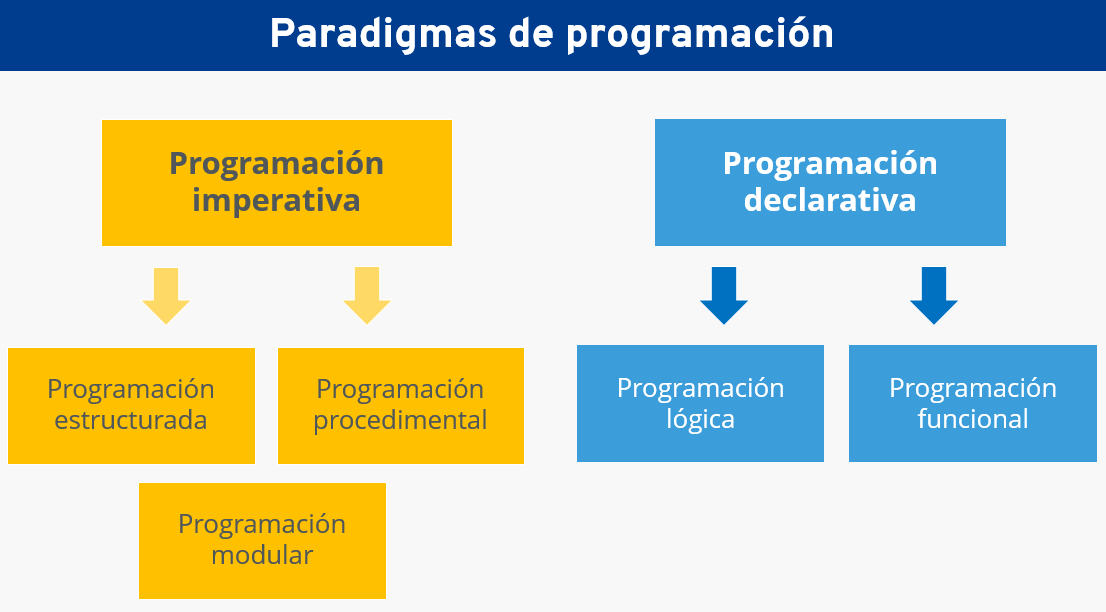
\includegraphics[scale=0.20]{./Paradigmas.png}
\end{center}
\subsection*{Parádigma Imperativo}
\begin{itemize}
\item \textbf{Orientado a objetos.} 
\item \textbf{Procedural.}
\item \textbf{Modular.}
\end{itemize}
\subsection*{Parádigma Declarativo}
\begin{itemize}
\item \textbf{Funcional.}
\item \textbf{Lógico.}
\end{itemize}
\hfill $\lhd$
